\chapter{Environments}
The sections of this chapter provide additional details about the custom environments used in our experiments.
Both of these environments were developed in Python.

\section{ShapeGridWorld}
\label{sec:sgw-details}
% Added color
% Added object_persistency 0
% Added step_size > 1
% Improved rendering
% Added partial reset with control and control boundaries
% Added controlled reset with max_dist
% Added partial control with control and control boundaries
\tabref{tab:original-sgw-params} lists the parameters of the original ShapeGridWorld environment developed by \cite{rair}.
\begin{table}[H]
    \centering
    \begin{tabularx}{\textwidth}{C{4.2cm} L}
        \hline
        Property & Description\\
        \hline
        \texttt{width} & Width of the discrete grid.\\
        \texttt{height} & Height of the discrete grid. Kept same as \texttt{width}.\\
        \texttt{n\_pixels} & Number of ``On'' pixels.\\
        \texttt{shape} & Shape of a pixel block -- ``circle''.\\
        \texttt{size} & Size of a pixel block.\\
        \texttt{persistency} & Number of time steps an object (pixel block) is moved. \\
        \hline
    \end{tabularx}
    \caption{Original ShapeGridWorld Parameters}
    \label{tab:original-sgw-params}
\end{table}
The state space of this environment is composed of the \(x\) and \(y\) coordinates of the \(n\) block pixels, with the addition of two dimensions -- one that specifies which object is currently in focus and another that specifies how many times it has already moved, i.e. \(\cS \in \nN^{2 n + 2}\).
The observation space is a rendering of the grid as an image of shape \(\texttt{width} * \texttt{size} \times \texttt{height} * \texttt{size}\).

The action space comprises the action value for each of the directions (x and y) for an object; \(\cA \in [-1, 1]^{2 n}\).
For each dimension, the controller samples from a continuous distribution in \([-1, 1]\), which is uniformly mapped to \(\{-1, 0, 1\}\) (\([-1, -1/3) \mapsto -1, [-1/3, 1/3] \mapsto 0, (1/3, 1] \mapsto 1\)).

We further added more features to this environment for our experiments, which are listed in \tabref{tab:additional-sgw-params}.
In particular, the ability to move all objects at once and more than one step in an action step was added.
We also developed a controlled reset method with the added feature to freeze sections of the grid, with \texttt{control} and \texttt{control\_boundaries}.
This additionally enabled us to allow the controller only partial access to the environment.
Furthermore, the rendering function was reimplemented using faster methods from \emph{OpenCV}; see \secref{sec:improving-render} for more details.

\begin{table}[h]
    \centering
    \begin{tabularx}{\textwidth}{C{4.2cm} L}
        \hline
        Property & Description\\
        \hline
        \texttt{step\_x} & Maximum number of steps an object can be translated in the x-direction in one action.\\
        \texttt{step\_y} & Maximum number of steps an object can be translated in the y-direction in one action. Kept same as \texttt{step\_x}.\\
        \texttt{persistency*} & Added the ability to move all objects at once.\\
        \texttt{color} & Grayscale value of the pixel. \\
        \texttt{control\_boundaries} & If specified, objects inside these limits \emph{initially} are marked.\\
        \texttt{control} & A flag that indicates whether the controller can move all the objects or those marked initially by the control boundaries.\\
        \texttt{max\_reset\_dist} & Maximum distance an object can be moved from its original position on reset. Only the objects marked initially are reset.\\
        \hline
    \end{tabularx}
    \caption{Additional ShapeGridWorld Parameters}
    \label{tab:additional-sgw-params}
\end{table}

If all objects are moved at once, the state space of this environment is composed of only the \(x\) and \(y\) coordinates of the block pixels, i.e. \(\cS \in \nN^{2 n}\).
The corresponding action space in this case would be \(\cA \in [-1, 1]^{2 n}\).
For each dimension of the action space, the controller samples from a continuous distribution in \([-1, 1]\), which is uniformly mapped to integers \([-l, l]\), where \(l \in \{\texttt{step\_x}, \texttt{step\_y}\}\) is the step size of the dimension.

\subsection{ShapeGridWorld Image Registration Technique}
\label{sec:sgw-registration}

To test CLIP inference on ShapeGridWorld and simulate the controller on partial drawings, without having to draw these drawing samples manually, a registration method for images was developed that reads a given image to generate a corresponding ShapeGridWorld of given dimensions.

This is done using a circular convolution kernel over the image to find the corresponding grid pixel values.
Optionally, it makes the lines in the image thinner by finding its skeleton using morphological operations before the convolution.
See \figref{fig:sgw-registration} for a demonstration.

\begin{figure}[h]
    \centering
    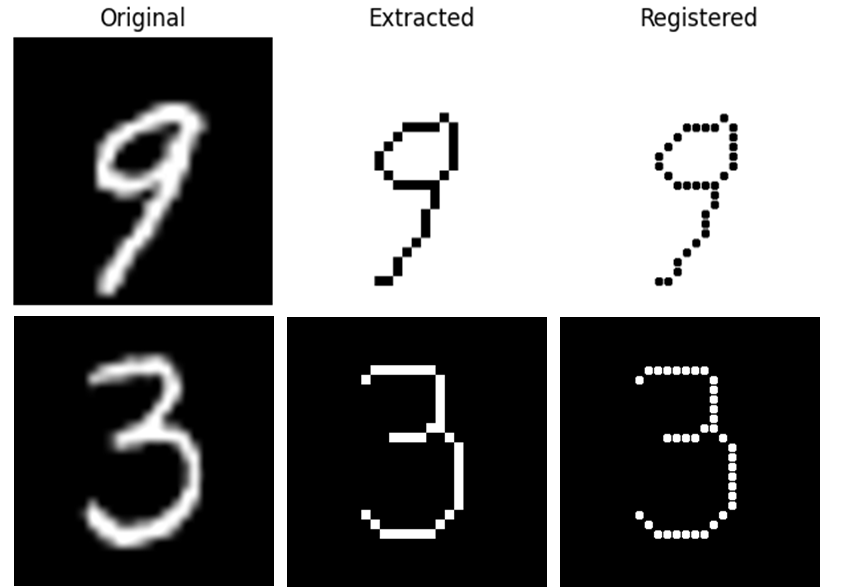
\includegraphics[width=0.7\textwidth]{images/grid_registration.png}
    \caption{ShapeGridWorld image registration on images from the MNIST dataset.}
    \label{fig:sgw-registration}
\end{figure}

The relevant code is hosted on \url{https://github.com/pulkitgoyal56/ImageGrid}.

\newpage
\section{Tangram}
\label{sec:tangram-details}
% flip
% rotate
% x_size
% r_size
% x_step
% object_persistency
% max_dist
% control
% control_boundaries
% staging_boundaries

The Tangram environment is initialized with a list of polygon objects created using the provided Polygon class, which define a polygon's size, shape, and color.
The additional parameters of the Tangram environment are tabulated in table \tabref{tab:tangram-params}.
\begin{table}[H]
    \centering
    \begin{tabularx}{\textwidth}{C{4.2cm} L}
        \hline
        Property & Description\\
        \hline
        \texttt{x\_size} & Span of the discrete grid; number of steps in the x-direction. If set to \(1\), grid is continuous in \([0, 1]\).\\
        \texttt{y\_size} & Span of the discrete grid; number of steps in the y-direction. If set to \(1\), grid is continuous in \([0, 1]\). Kept same as \texttt{x\_size}.\\
        \texttt{r\_size} & Span of the discrete grid; number of rotation steps in \(360^\circ\). If set to \(1\), rotation is continuous in \([0, 360^\circ]\).\\
        \texttt{x\_step} & Maximum number of steps a polygon can be translated in the x-direction in one action.\\
        \texttt{y\_step} & Maximum number of steps a polygon can be translated in the y-direction in one action. Kept same as \texttt{y\_step}.\\
        \texttt{r\_step} & Maximum number of steps a polygon can be rotated in one action.\\
        \texttt{rotation} & A flag to enable/disable rotation.\\
        \texttt{flip} & A flag to enable/disable flipping.\\
        \texttt{persistency} & Number of time steps a polygon (pixel block) is moved. If set to \(1\), all polygons are moved at once.\\
        \texttt{control\_boundaries} & If specified, polygons inside these limits \emph{initially} are marked.\\
        \texttt{control\_criteria} & The point inside the polygon used to determine if the polygon is inside or outside the control boundaries. Can be a Python lambda function or an attribute of a polygon, such as ``centroid'', ``center'', or ``complete''.\\
        \texttt{control} & A flag that indicates whether the controller can move all the polygons or those marked initially by the control boundaries.\\
        \texttt{staging\_boundaries} & If specified, only polygons inside these limits are rendered to get the state's corresponding image observation.\\
        \texttt{staging\_criteria} & Similar to \texttt{control\_criteria} but for staging boundaries.\\
        \texttt{max\_reset\_dist} & Maximum distance a polygon can be moved from its original position on reset. Only the polygons marked initially are reset.\\
        \hline
    \end{tabularx}
    \caption{Tangram Parameters}
    \label{tab:tangram-params}
\end{table}

The state space of this environment is composed of the \(x\) and \(y\) coordinates of the vertices of the \(n = 7\) polygons, with the addition of two dimensions -- one that specifies which polygon is currently in focus and another that specifies how many times it has already moved, i.e. \(\cS \in \nN^{\,2 + \sum_{i \in n} 2\ n_v(p_i)}\), where \(n_v(p_i)\) is the number of vertices of polygon \(p_i\).
If all polygons are moved at once, the state space of this environment is composed of only the \(x\) and \(y\) coordinates of the block pixels, i.e. \(\cS \in \nN^{\sum_{i \in n} 2\ n_v(p_i)}\).
The observation space is a rendering of the grid whose resolution is controlled with different parameters.

The action space comprises the action value for each of the degrees of freedom (x, y, rotation, and flip) for an object; \(\cA \in [-1, 1]^4\).
For each dimension of the action space, the controller samples from a continuous distribution in \([-1, 1]\).
In the x-, y-, and rotation dimensions, this is uniformly mapped to integers in \([-l, l]\), where \(l \in \{\texttt{step\_x}, \texttt{step\_y}, \texttt{step\_r}\}\) is the step size of the dimension, if it is discrete.
If the dimension is continuous (because its \texttt{size} is set to \(1\)), the action is scaled by its respective step size instead.
For example, if \texttt{x\_size} is \(1\) and \texttt{x\_step} is \(3\), the resulting support of the action distribution for any action sampled for x-dimension will be \([-1/3, 1/3]\).
For the flip dimension, the mapping is (\([-1, 0] \mapsto \texttt{False}, (0, 1] \mapsto \texttt{True}\)).

The developed code to create Tangram-like environments with any number of arbitrary convex polygons is available on \url{https://github.com/pulkitgoyal56/Tangram}.


\chapter{Flatnet}
\label{sec:flatnet}
To test the feasibility and efficacy of fine-tuning CLIP with an entropy regularization technique to reduce its inference noise, we conducted some experiments on a smaller toy setup with convolutional neural networks trained as an MNIST classifier.


% \chapter{Descriptive List of Main Hyperparameters}
% \label{sec:hyperparameters}
% Here, we provide a list of the hyperparameters we mainly considered in our experiments.


\chapter{Improving Simulation Times}
\label{sec:efficiency}
Rendering the environment and using CLIP for planning was a very resource-intensive operation.
At every planning step, a total of \(\text{n\_trajectories} \times \text{horizon} \times \text{n\_icem\_inner\_iterations}\) evaluations needed to be computed.
This was further multiplied by the number of steps in the simulation.
This total ranged anywhere from \(~200,000\) to \(~2,000,000\) in our many experiments which corresponded to about \(2\) to \(20\) hours of simulation time if run in a single batch of inference on multiple GPUs.

Reducing this time was critical for us to be able to do any hyperparameter analysis properly.
We implemented several optimization strategies to improve this, which mainly involved \emph{vectorization} of all computation, parallelization, and cutting down on redundant operations.
In particular, two of these optimizations, for rendering and inference, are briefly introduced in the sections of this appendix chapter.

\section{Reducing Rendering Time}
\label{sec:improving-render}
The rendering time was a major bottleneck for the simulations.
To improve this, we experimented with three popular open-source graphics Python libraries; \emph{Matplotlib} \citep{matplotlib}, \emph{Scikit-Image} \citep{skimage}, and \emph{OpenCV} \citep{opencv}, for colored and grayscale renderings.
We used their functions in different formulations to further optimize their use.
The results of the best formulation for each of these libraries are summarized in \tabref{tab:render-time-color} and \tabref{tab:render-time-bw}.\\

\begin{table}[H]
    \centering
    \begin{tabular}[t]{@{} c c c @{}}
        \hline
        \textbf{Library} & \textbf{Main Function/Class} & \textbf{Time (\(\mu s\))*}\\
        \hline
        Matplotlib & \texttt{PatchCollection} & 14400 ± 153\\
        Scikit-Image & \texttt{draw.polygon} & 978 ± 10.8\\
        OpenCV & \texttt{fillPoly} & 66.3 ± 0.85\\
        \hline
    \end{tabular}
    \caption{Colored Rendering Time Comparison}
    \label{tab:render-time-color}
\end{table}
\begin{table}[H]
    \centering
    \begin{tabular}[t]{@{} c c c @{}}
        \hline
        \textbf{Library} & \textbf{Main Function/Class} & \textbf{Time (\(\mu s\))*}\\
        \hline
        Matplotlib & \texttt{PatchCollection} & 14200 ± 156\\
        Scikit-Image & \texttt{draw.polygon} & 978 ± 10.8\\
        OpenCV & \texttt{fillConvexPoly} & 52.2 ± 1.04\\
        \hline
    \end{tabular}
    \caption{Grayscale Rendering Time Comparison}
    \label{tab:render-time-bw}
\end{table}
* - Mean \(\pm\) standard deviation of \(7\) runs; \(1,000 - 10,000\) loops each.

These results refer to the Tangram environment, but the trend was the same with ShapeGridWorld.
The complete analysis is available on \url{https://github.com/pulkitgoyal56/master-thesis-notebooks/blob/main/archive/testbed_rendering.ignore.ipynb}.

\section{Reducing Inference Time}
\label{sec:improving-infer}
To minimize the inference times with CLIP, all inferences were done in one large batch.
This required significant memory, for which we parallelized them on multiple GPUs using Pytorch \texttt{DataParallel} \citep{pytorch}.
Depending on their size, the simulations were run concurrently on multiple NVIDIA V100 and A100 GPUs.

To reduce the inference time, we tweaked the image preprocessing functions of CLIP to be adaptive to the input to ensure that no redundant operations were performed.

Furthermore, we typically chose the rendering configurations for the environments such that the resulting renders did not require any preprocessing in the form of resizing, cropping, type conversions, or copying, which was computationally expensive.
For example, all renderings concurred with the required input for the used CLIP model (eg. \(224 \times 224\) for the \texttt{ViT-L/14} variant) used for inference to avoid any resizing.
This also helped to improve the simulation times significantly.\\

\begin{figure}[H]
    \centering
    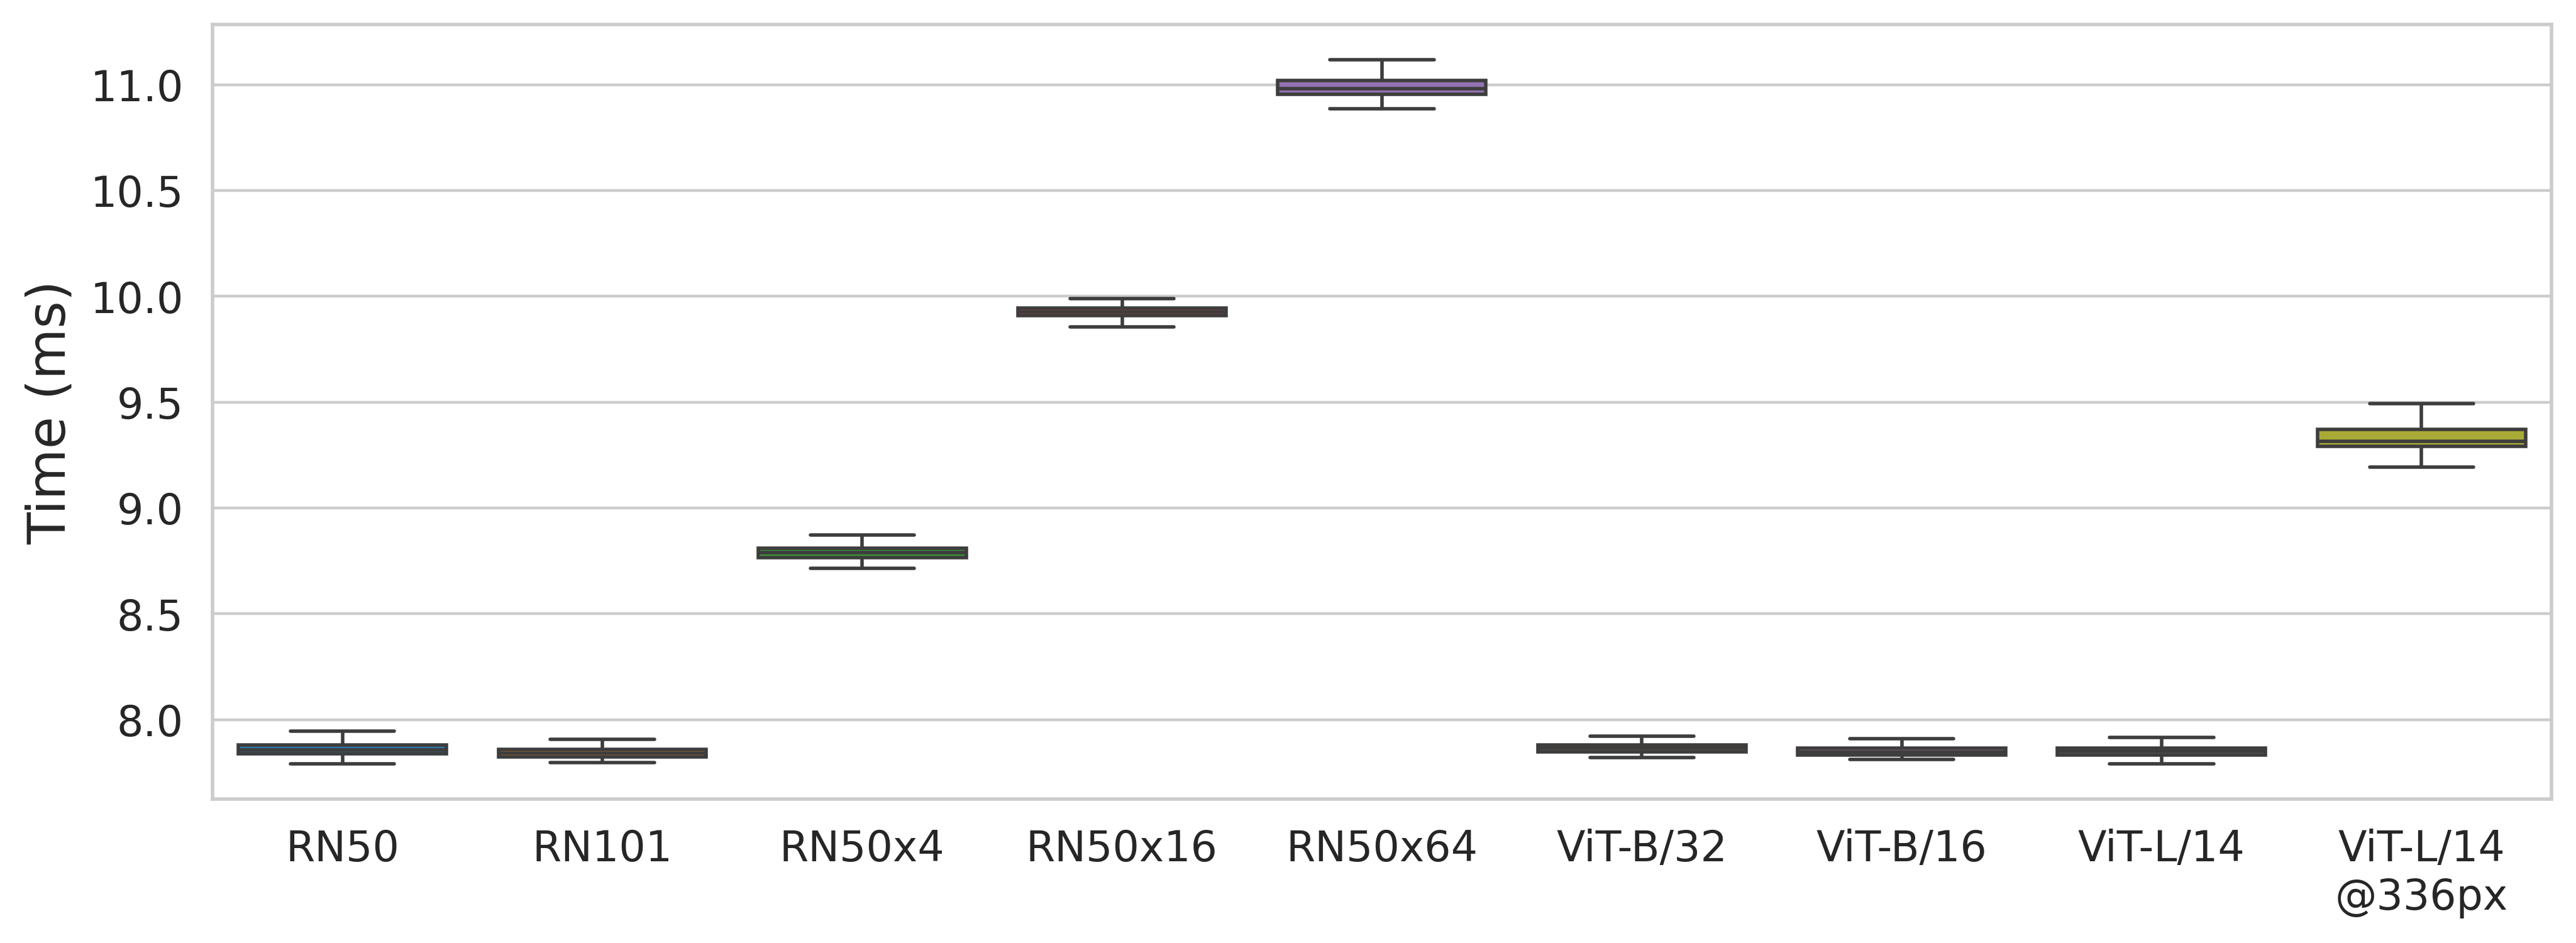
\includegraphics[width=\textwidth]{images/full_transform.png}\vspace{-15pt}
    \caption{Preprocessing times before optimizations.}\vspace{15pt}
    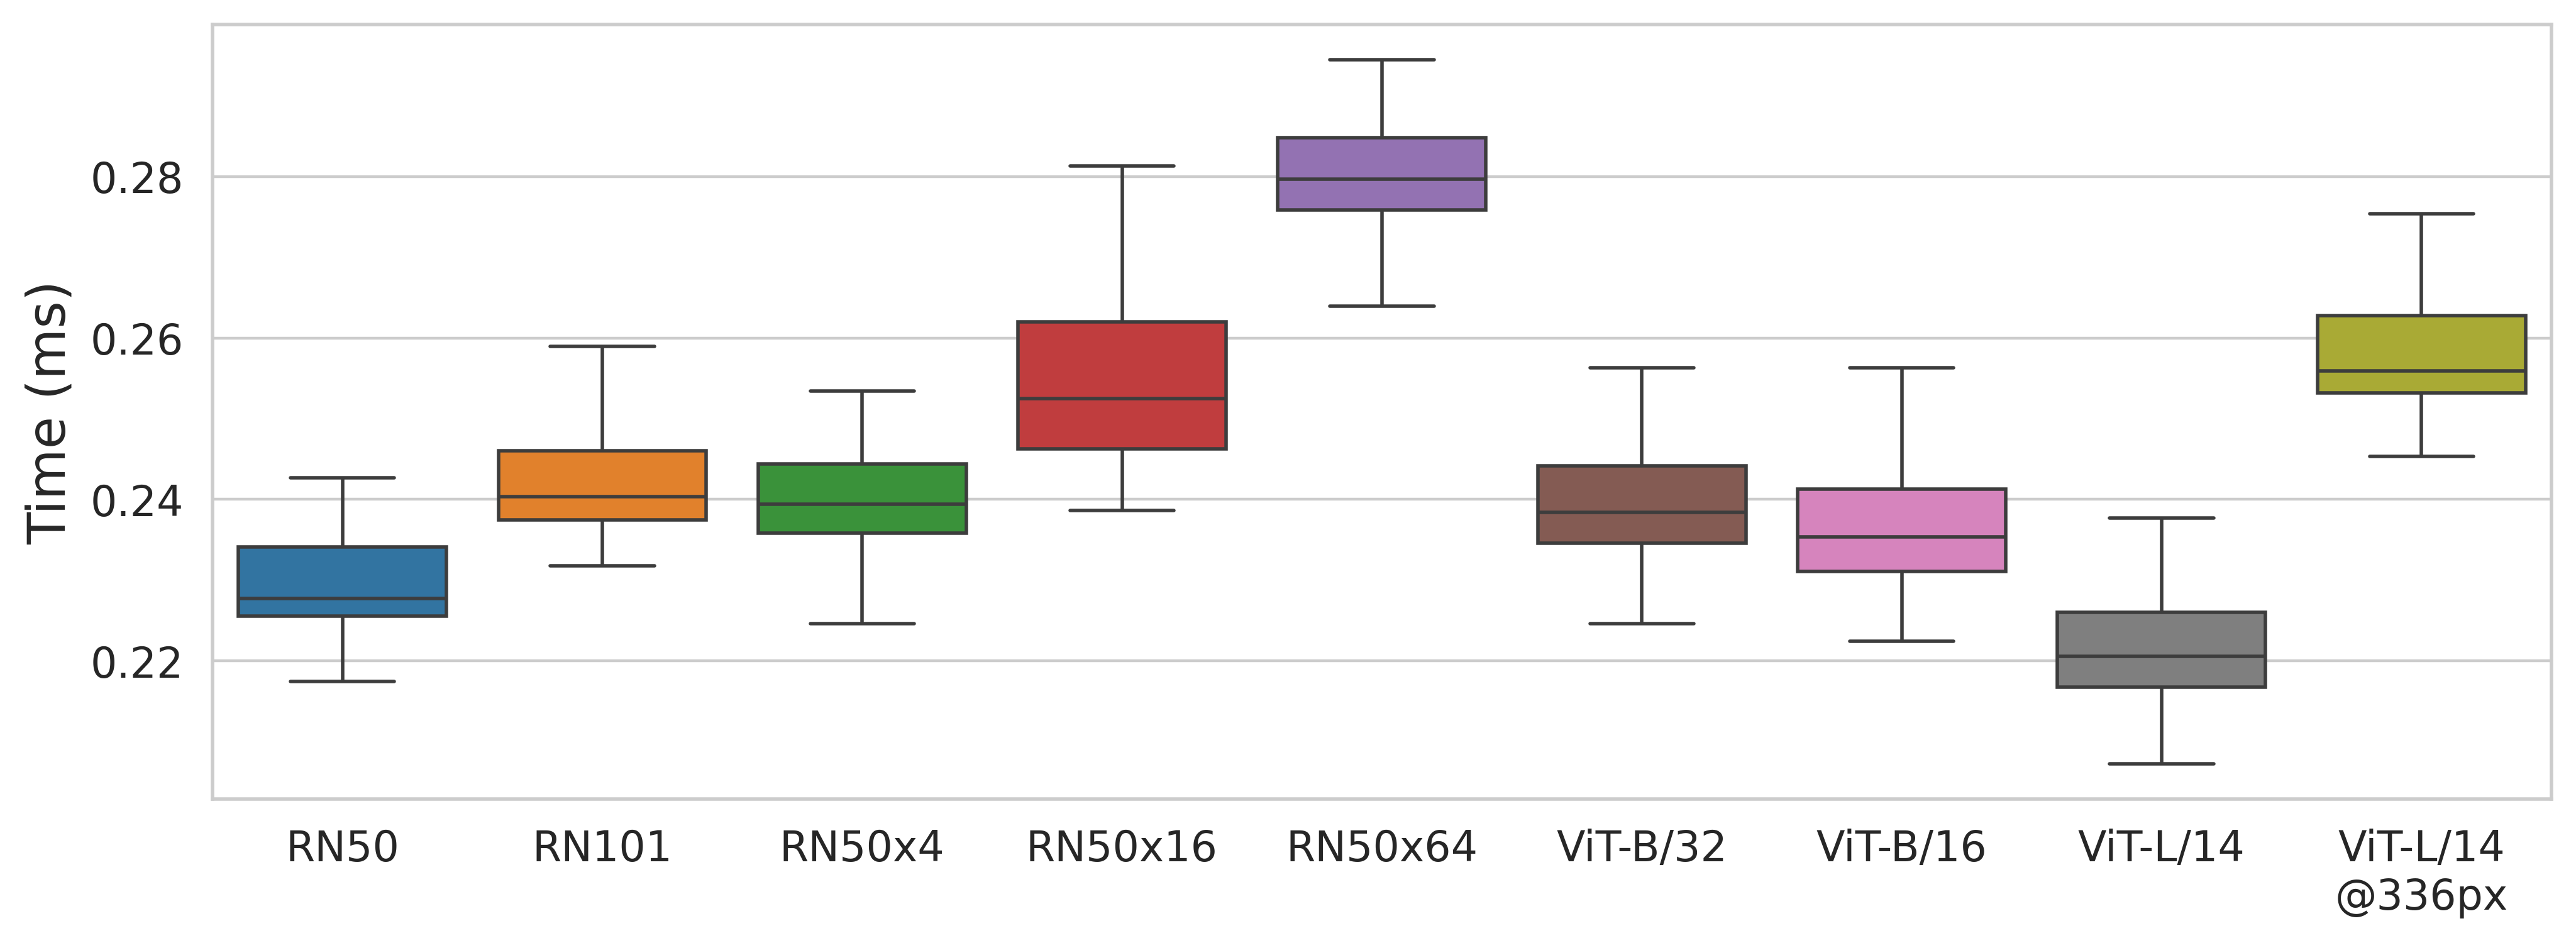
\includegraphics[width=\textwidth]{images/fast_transform.png}\vspace{-15pt}
    \caption{Preprocessing times after optimizations.}
    \label{fig:preprocessing-time-improvement}
\end{figure}

These modifications are available on \url{https://github.com/pulkitgoyal56/CLIP/tree/preprocess-tweaks}.
